\section{Implementation}\label{sec:implementation}
% section conclusion
This section contains the Colladoc Smart Search implementation details. We outline the main implementation choices and explain the reasons for them. 

The original Colladoc uses Lift 2.0 as for web application framework. In extending Colladoc, we followed that. Colladoc uses a MVVM pattern \cite{lift} \emph{\color{red} why the star is here?}, which means that the application is split into a Model - View - ViewModel which map closely to our Model - UI - Query layers respectively.

The MVVM pattern is classic three-layer application pattern similar to MVC and MVP. In the MVVM pattern the Model contains data; the ViewModel contains the business logic. It also matches the View closely in structure and handles events coming from the View; The View visualises the ViewModel.
\begin{figure}[h!t]
\begin{center}
\leavevmode
{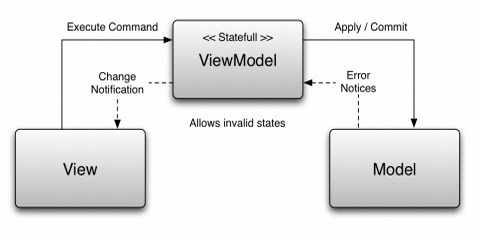
\includegraphics[width=0.9\textwidth]{mvvm}}
\end{center}
\caption{MVVM as explained in \cite{lift}}
\label{fig:mvvm}
\end{figure}

\subsection*{Model Layer}
For the data indexing we used Apache Lucene, an open source search engine. Our team member – Rumyana Neykova – had prior experience with it and Lucene was the suggested indexing technology in the initial project proposal, so we did not consider any other search engines.

\textbf{When we index}\\ 
The indexing is done by the $SearchIndexer$ class. We agreed on synchronously indexing the entire documentation model right after it is constructed (i.e. when the application is launched) to eliminate the overhead when performing searches. Although we considered other indexing strategies such as waiting for the first query to index or indexing the documentation model asynchronously, those were rejected because in the first case the delay would be noticeable by the user and in the second queries executed before indexing completed would have produced incomplete results. The documentation model does not change often, so indexing upfront is justified.

The only time when the search index needs to be updated is when a user edits the documentation. Therefore, the $SearchIndexer$ has the ability to re-index individual symbols. We  obtained acceptable  performance by making the reindexing right after the user saves an edit to the documentation.

\textbf{What do we index}\\
The documentation model is indexed and stored with the help of the Lucene search engine. 
Lucene stores its contents in separate units called ‘documents’. Each document has searchable text contents. Documents are returned as a result of querying the Lucene database. The structure of the document that we stored was very important since it affects what search queries we can make and what results are returned. Therefore, we had to decide whether to have one document per class or one document per class member. Two of us (Miroslav Paskov and Jamil Rzaev) worked on the functionality in parallel for a week. It showed that storing separate documents gives us more granular results and makes the individual documents simpler, without any performance overhead. From development and maintenance perspective this was a better choice and we decided to have a more granular indexing. This decision meant that we needed to match each class member to its respective class. Lucene does not support document relations by default so we did this by assigning a unique id to each entity of the documentation model and its respective Lucene document. 

\textbf{Lucene 3.0 or Lucene 4.0}\\
Initially, we started using Lucene 3.0 as it is the latest released version of Lucene. After the project was underway we realized that the coming version of Lucene, 4.0, is a better candidate for our purpose since it allowed more precise queries to be made. Unlike Lucene 3.0, the new version does not suffer from performance drawbacks with wild-card queries (e.g. [q5], [q11]) which we expect to be often used in searches. For one week, two of us (Miroslav Paskov and Jamil Rzaev) did parallel development in both Lucene 3.0 and 4.0 to make sure that we meet the iteration’s objectives and to mitigate any potential transition problems. This was duplication of efforts but in the end we could make an objective decision to adopt Lucene 4.0.

\subsection*{Query Layer}

The $SearchSnippet$ maps to the ViewModel in the Lift MVVM pattern.

When the user enters a search query it is parsed by the $QueryParser$ class to an abstract syntax tree (AST) of the search query ($SearchQuery$ class and its descendants). This AST is search-engine independent and contains all information for the search query. It is transformed to a Lucene-specific query object (an instance of Query).

\textbf{Query Parsing or Direct Transformation} 
Simple wildcard queries (containing * or ?) can be directly transformed to a syntax that is supported by the Lucene search engine. In our initial discussion we were aiming for this approach. Early on, we agreed that we need to support complex syntax, for example:

\begin{lstlisting}
(List[_], _Map, *) => (Int, String)
\end{lstlisting}

We needed to distinguish language features such as generics, lambda parameters and tuples. This required a parser that can handle this syntax and give us more flexibility. We looked into several options for a parsing, in the first weeks of development. 

\textbf{Custom, Generated or Combinatorial Parser}\\
We started with an ad-hoc implementation of a parser. After one week it could distinguish the first three basic queries but it looked like continuing in the same style will prove to be increasingly difficult to develop and maintain. We were aware of parser generators like ANTLR or JavaCC but we expected that Scala, being partly functional, may have a language feature or library that helps parsing. We came across Combinatorial Parsers – which are a built-in library that allows defining parsers succinctly, very much like a BNF(*) grammar, for example:

\begin{lstlisting}
def expr = or | and  | term
def `val` = "val" ~> identifier ~ returnType
\end{lstlisting}
We were very happy with the clarity and expressiveness of the library and we chose it for the parser.

\textbf{How Results are Ordered}\\ 
The default ordering implemented by Lucene is used. Lucene uses result weights to determine which results come first. Result weights are calculated based on how often a word occurs in the document or whether queried terms are near each other. Only searching for text in comments produces varying result weights - this is due to how we index the documents. All other searches produce results with equal relevance.
UI Layer 

The $SearchPage$ maps to the View in the Lift MVVM pattern. Views are combination of dynamic inline HTML that renders the information in browsers. 

\textbf{Reusing Scaladoc and Colladoc UI Templates}\\
Initially we did not know how much of the existing UI code could be reused but we started work on the UI with the intention of reusing as much as possible. Thus we preserved much of the look-and-feel of Scaladoc in our results page. We reused templates for page headers, displaying results and filtering results. 

\textbf{Inline Html}\\
As a rule, we followed the existing coding style. Our UI code contains inline HTML literals which may not be a good coding practice but it made our new code consistent with existing code. We decided it was more important to follow the existing coding style for maintainability and not introduce a new one.

\textbf{Infinite Scrolling (Lazy loading) or Pagination}\\
Infinite scrolling is a UI pattern where only a part of a longer content will be initially loaded. When the user scrolls down to reveal more content, it gets asynchronously loaded. Initially, we decided to implement pagination for longer search results then we agreed that infinite scrolling gives better user experience. It allows the user to continue to view content on a single page without having to leave it. No clicks are needed to load more information on the page.

\textbf{Implementing Infinite Scrolling}\\
We had the option to either use an existing infinite scrolling library or implement it ourselves. It turned out that existing libraries did not fit very well with our current implementation and it would be easier to implement it ad-hoc.

The infinite scrolling has two major elements:
\begin{enumerate}
\item The Lucene IterablePagingCollector class which only reads a subset of all results for a query.
\item A jQuery script - that listens for when the page is scrolled to the bottom and makes an AJAX call for the continuation of the results, depending on how many results have been retrieved so far.
\end{enumerate}
